\documentclass[tikz]{standalone}
\usetikzlibrary{arrows,shapes,automata,petri,positioning}

\tikzset{
	place/.style={
		circle,
		very thick,
		draw=blue!90,
		fill=blue!10,
		minimum size=6mm,
	},
	transitionH/.style={
		rectangle,
		thick,
		fill=black,
		minimum width=6mm,
		inner ysep=2pt
	},
	transitionV/.style={
		rectangle,
		thick,
		fill=black,
		minimum height=6mm,
		inner xsep=2pt
	},
    tau/.style={
      fill=gray,
    },
    arc/.style={
        -triangle 45,
        thick,
    }
}


\begin{document}
	
	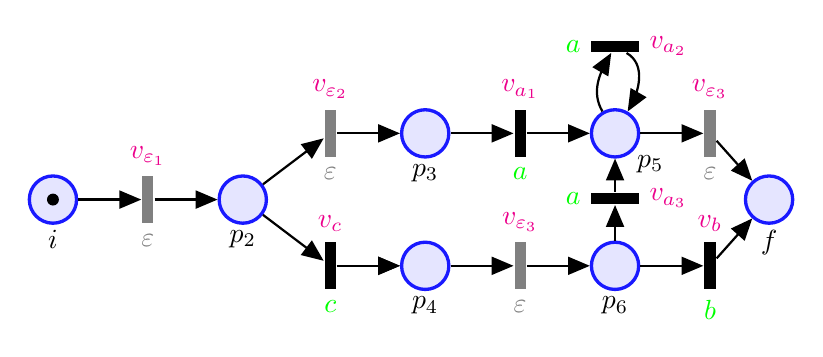
\begin{tikzpicture}[node distance=0.3cm and 0.8cm,>=stealth',bend angle=45,auto]
	\node [place,tokens=1] (i) {};
    \node [below=-0.5mm of i] {$i$};
	\node [
      transitionV,
      tau,
      right= of i,
      label=below:$\color{gray}\varepsilon$,
      label=above:$\color{magenta}v_{\varepsilon_1}$,
    ] (t1) {};
	\node [
      place,
      right=of t1
    ] (p2){};
    \node [
      below=-0.5mm of p2
    ] {$p_2$};
	\node  (b1) [right=of p2] {};
	\node  (b2) [right=of b1] {};
	\node [
      transitionV,
      tau,
      above right=of p2,
      label=below:$\color{gray}\varepsilon$,
      label=above:$\color{magenta}v_{\varepsilon_2}$,
    ] (te1) {};
	\node [
      place, 
      right=of te1
    ] (p3) {};
    \node [
      below=-0.5mm of p3
    ] {$p_3$};
    \node [
      transitionV,
      right=of p3,
      label=below:$\color{green}a$,
      label=above:$\color{magenta}v_{a_1}$,
    ] (ta1) {};
	\node [
      place,
      right=of ta1
    ] (p5) {};
    \node [
      below right=-1mm of p5
    ] {$p_5$};
    \node [
      transitionH,
      above=of p5,
      label=left:$\color{green}a$,
      label=right:$\color{magenta}v_{a_2}$,
      yshift=4mm
    ] (ta2) {};
	\node [
      transitionV,
      tau,
      right=of p5,
      label=below:$\color{gray}\varepsilon$,
      label=above:$\color{magenta}v_{\varepsilon_3}$,
    ] (te2) {};
	\node [
      transitionV,
      below right=of p2,
      label=below:$\color{green}c$,
      label=above:$\color{magenta}v_{c}$
    ] (tc1) {};
	\node [
      place,
      right=of tc1
    ] (p4) {};
    \node [
      below=-0.5mm of p4
    ] {$p_4$};
	\node [
      transitionV,
      tau,
      right=of p4,
      label=below:$\color{gray}\varepsilon$,
      label=above:$\color{magenta}v_{\varepsilon_3}$
    ] (te3) {};
	\node [place] (p6) [right=of te3] {};
    \node [below=-0.5mm of p6] {$p_6$};
	\node [
      transitionV,
      label=below:$\color{green}b$,
      label=above:$\color{magenta}v_b$
    ] (tb1) [right=of p6] {};
	\node  (b3) [right=of b2] {};
	\node  (b4) [right=of b3] {};
	\node  (b5) [right=of b4] {};
	\node [place] (f) [right=of b5] {};
    \node [below=-0.5mm of f] {$f$};

    \node [
      transitionH,
      above=4.5mm of p6,
      label=left:$\color{green}a$,
      label=right:$\color{magenta}v_{a_3}$,
    ] (ta3) {};
    
    \draw[arc] (i) -- (t1);
    \draw[arc] (t1) -- (p2);
    \draw[arc] (p2) -- (te1);
    \draw[arc] (te1) -- (p3);
    \draw[arc] (p3) -- (ta1);
    \draw[arc] (ta1) -- (p5);
    \draw[arc,out=120,in=-120] (p5) edge (ta2);
    \draw[arc,out=-30,in=60] (ta2) edge (p5);
    \draw[arc] (p5) -- (te2);
    \draw[arc] (te2) -- (f);

    \draw[arc] (p2) -- (tc1);
    \draw[arc] (tc1) -- (p4);
    \draw[arc] (p4) -- (te3);
    \draw[arc] (te3) -- (p6);
    \draw[arc] (tc1) -- (p4);
    \draw[arc] (p6) -- (tb1);
    \draw[arc] (tb1) -- (f);

    \draw[arc] (p6) -- (ta3);
    \draw[arc] (ta3) -- (p5);
    
	\end{tikzpicture}
	
\end{document}